%----------------------------------------------------%
%              DISEÑO E IMPLEMENTACIÓN               %
%----------------------------------------------------%

\chapter{Diseño e Implementación}
\label{diseno-e-implementacion}

Añadir descripcion del apartado.\\

\section{Estructura del proyecto}
\label{diseno-e-implementacion:estructura}

En este apartado se revisara la estructura del proyecto, es decir, los ficheros que componen el proyecto y su estructura de carpetas. En la figura ~\ref{fig:files-1} se muestra la raíz del proyecto:\\

\begin{figure}[h]
	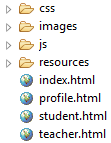
\includegraphics{files-1}
	\caption{Raíz del proyecto}
	\label{fig:files-1}
\end{figure}

El proyecto cuenta con 4 carpetas principales: css, js, images y resources. Además contiene 4 ficheros HTML:

\begin{itemize}
\item \textbf{index.html:} funciona como pantalla de identificación de usuario y permite redirigir a las vistas principales (teacher.html o student.html) dependiendo del rol del usuario identificado.
\item \textbf{student.html:} es la vista del alumno.
\item \textbf{teacher.html:} es la vista del profesor.
\item \textbf{profile.html:} pantalla de perfil del profesor, únicamente accesible desde teacher.html.
\end{itemize}

Estos ficheros muestran las interfaces principales de la aplicación. Dentro de las otras carpetas encontramos más ficheros.

\begin{figure}[h]
\begin{subfigure}[b]{0.5\textwidth}
	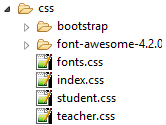
\includegraphics[width=0.6\linewidth]{files-css}
	\caption{Contenido de la carpeta css}
	\label{fig:files-css}
\end{subfigure}
%
\begin{subfigure}[b]{0.5\textwidth}
	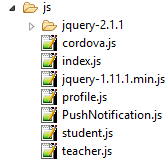
\includegraphics[width=0.6\linewidth]{files-js}
	\caption{Contenido de la carpeta js}
	\label{fig:files-js}
\end{subfigure}
%
\begin{subfigure}[b]{0.5\textwidth}
	
\includegraphics[width=0.6\linewidth]{files-images}
	\caption{Contenido de la carpeta images}
	\label{fig:files-images}
\end{subfigure}
%
\begin{subfigure}[b]{0.5\textwidth}
	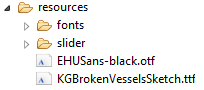
\includegraphics[width=0.6\linewidth]{files-resources}
	\caption{Contenido de la carpeta resources}
	\label{fig:files-resources}
\end{subfigure}

\caption{Contenido de la carpetas principales de la raíz del proyecto}
\label{fig:files-2}
\end{figure}

Los archivos de CSS sirve para darle estilo a las interfaces. Cada interfaz tiene un archivo .css asociado (excepto profile.html, que comparte teacher.css con teacher.html). Además, se añaden dos carpetas extra: la que necesitamos para Boostrap \hyperref[boostrap]{\cite{boostrap}} y para usar los iconos de Font Awesome \hyperref[fontawesome]{\cite{fontawesome}}.\\

Los ficheros Javascript de la carpeta JS le dan dinamicidad a la aplicación. Controlan los clicks, hacen aparecer las pestañas nuevas y cargan contenido dinámicamente mediante AJAX. Cada interfaz (fichero HTML) tiene asociado su propio fichero JS. Además se incluye el fichero cordova.js y los ficheros necesarios para utilizar JQuery.\\

La carpeta images contiene las imágenes utilizadas en el proyecto y la carpeta resources contiene otros elementos utilizados en el proyecto (en este caso fuentes utilizadas).\\

\section{Interfaces o lado del cliente}
\label{diseno-e-implementacion:interfaces}

En este apartado se mostrarán las interfaces desarrolladas partiendo de los modelos de requisitos (M-1) de cada objetivo y algunos elementos comunes de todos los objetivos.

\subsection{Interfaz de autenticación de usuario}
\label{diseno-e-implementacion:interfaces:autenticacion}

\begin{figure}[H]
	\centering
	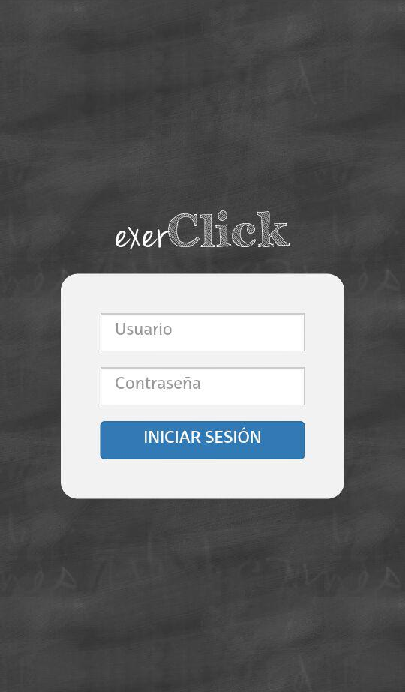
\includegraphics[height=7cm, frame]{autenticacion}
	\caption{Pantalla de autenticación de usuario}
	\label{fig:autenticacion}
\end{figure}

La pantalla de autenticación de usuario (index.html) de la figura ~\ref{fig:autenticacion} es la primera que se muestra al iniciar la aplicación. Esta pantalla nos redirige a teacher.html o student.html (vista del profesor y del alumno, respectivamente) dependiendo del rol del usuario con el que nos identifiquemos (el rol está definido en la base de datos).\\

\subsection{Interfaz del profesor}
\label{diseno-e-implementacion:interfaces:profesor}

\begin{figure}[H]
	\centering
	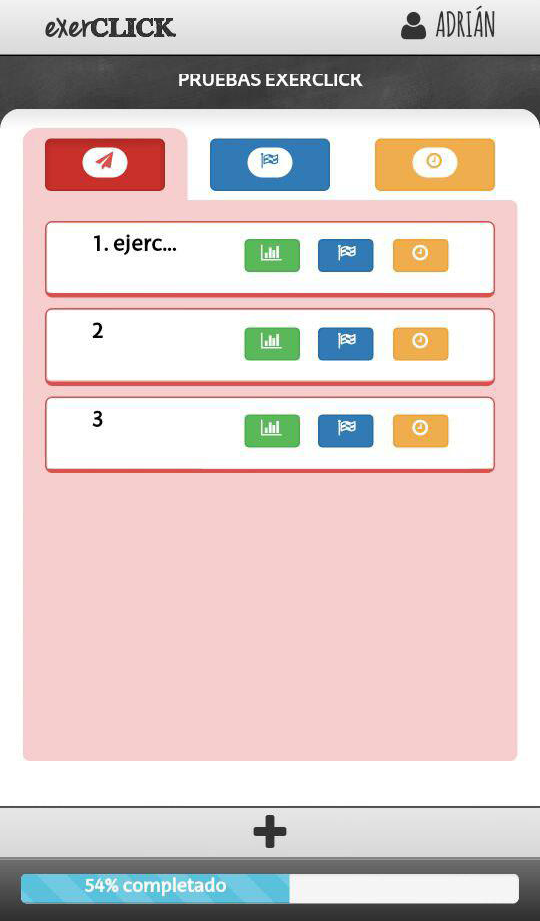
\includegraphics[height=7cm, frame]{activos}
	\caption{Pantalla en la que se muestran los ejercicios activos en clase}
	\label{fig:activos}
\end{figure}

La pantalla del profesor nos muestra el entorno de opciones del que dispone el docente.\\

\subsection{Interfaz del perfil del profesor}
\label{diseno-e-implementacion:interfaces:perfil}

\begin{figure}[H]
	\centering
	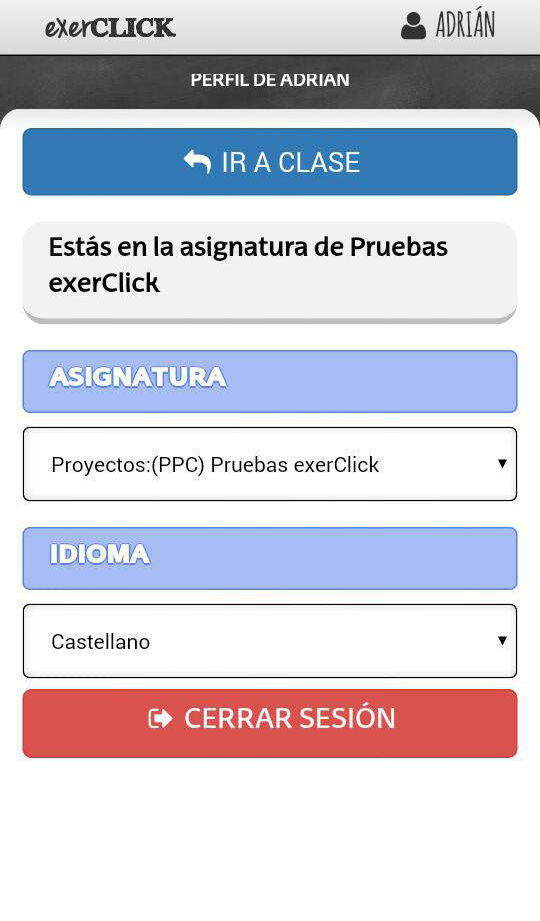
\includegraphics[height=7cm, frame]{perfil}
	\caption{Perfil del profesor}
	\label{fig:perfil}
\end{figure}

Es la interfaz de teacher.html, y la vista de profesor de inicio después de autenticarse. Esta pantalla sirve como base de cualquier UO del profesor, ya que hay que pasar obligatoriamente por ella.

\subsubsection{UO1-T: Crear-Lanzar un ejercicio simple}
\label{diseno-e-implementacion:interfaces:profesor:uo1-t}

\begin{figure}[H]
	\centering
	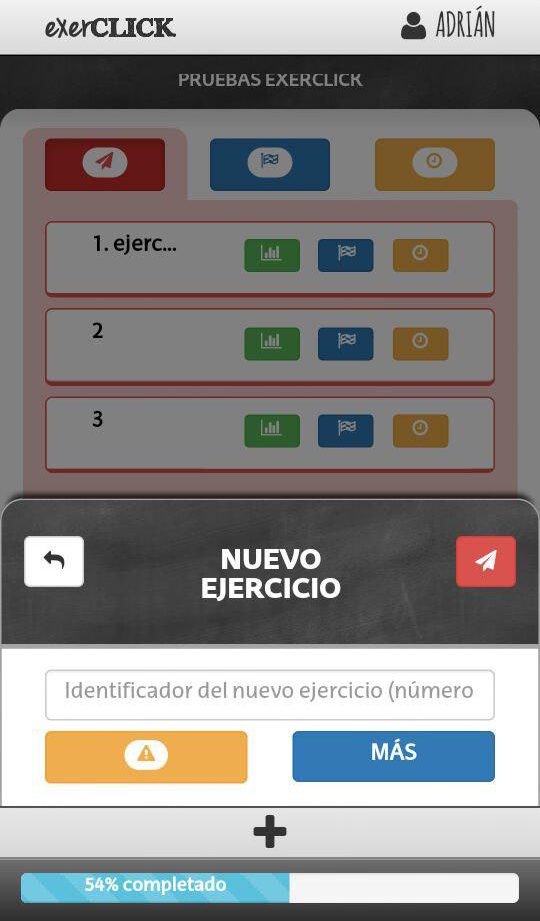
\includegraphics[height=7cm, frame]{ejercicio-simple}
	\caption{Interfaz del UO1-T: Crear-Lanzar un ejercicio simple}
	\label{fig:crear-lanzar-ejercicio-simple}
\end{figure}

Al pulsar el botón con símbolo de '+' (\textit{plus}/más) de la parte inferior de la interfaz del profesor se desplegará la pestaña que aparece en la figura ~\ref{fig:crear-lanzar-ejercicio-simple}.

\subsubsection{UO2-T: Crear-Lanzar un ejercicio detallado}
\label{diseno-e-implementacion:interfaces:profesor:uo2-t}

\begin{figure}[H]
	\centering
	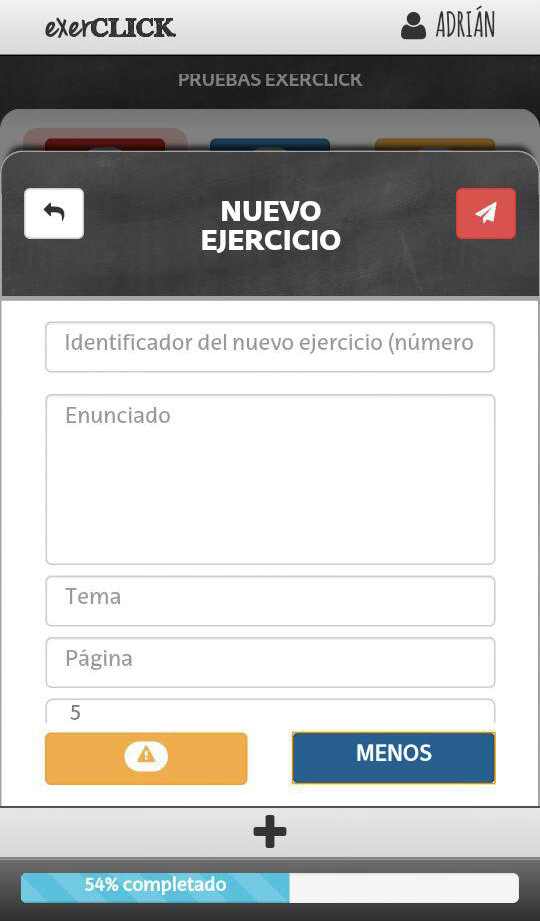
\includegraphics[height=7cm, frame]{ejercicio-avanzado}
	\caption{Interfaz del UO1-T: Crear-Lanzar un ejercicio detallado}
	\label{fig:crear-lanzar-ejercicio-avanzados}
\end{figure}

\subsubsection{UO4-T: Ver estadísticas de un ejercicio}
\label{diseno-e-implementacion:interfaces:profesor:uo4-t}

\begin{figure}[H]
\begin{subfigure}[b]{0.3\textwidth}
	\centering
	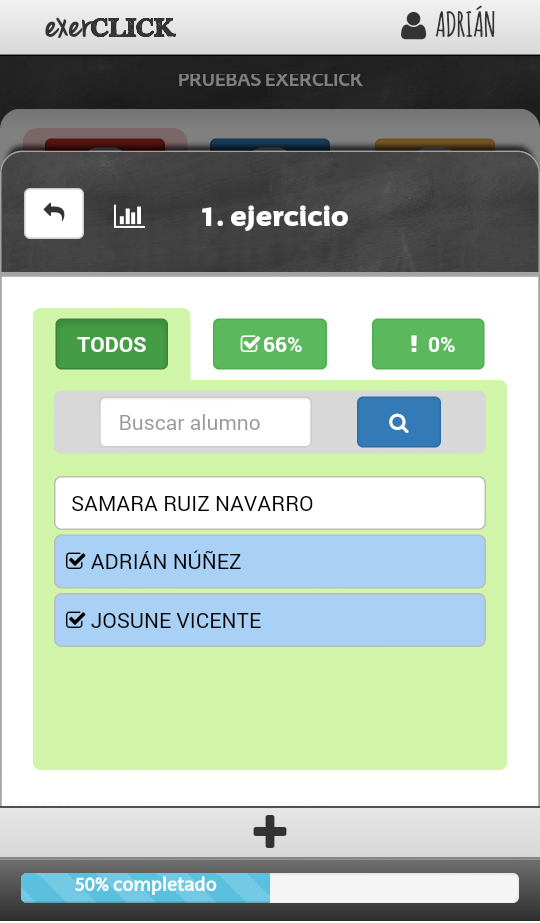
\includegraphics[height=7cm, frame]{P5T}
	\caption{P5T}
	\label{fig:req-autenticacion:p0}
\end{subfigure}
%
\begin{subfigure}[b]{0.3\textwidth}
	\centering
	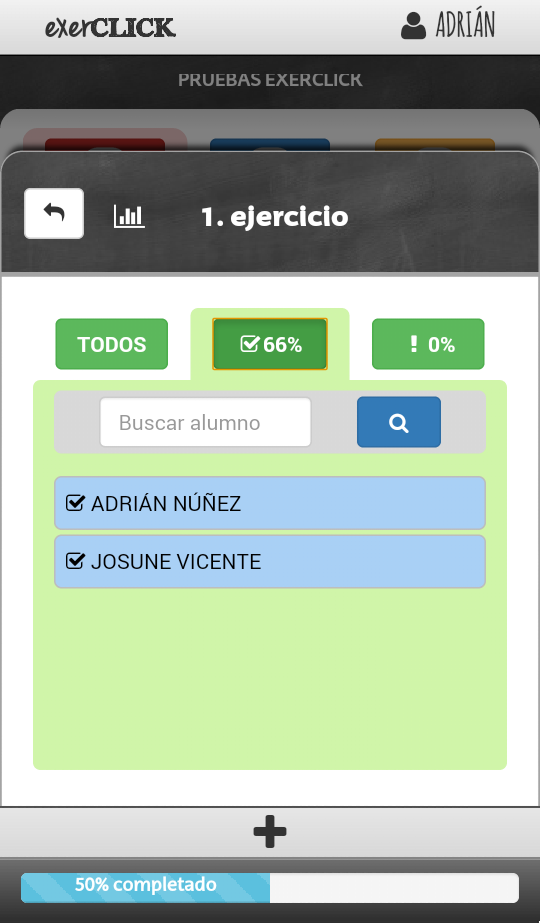
\includegraphics[height=7cm, frame]{P5A}
	\caption{P5A}
	\label{fig:req-autenticacion:p0'}
\end{subfigure}
%
\begin{subfigure}[b]{0.3\textwidth}
	\centering
	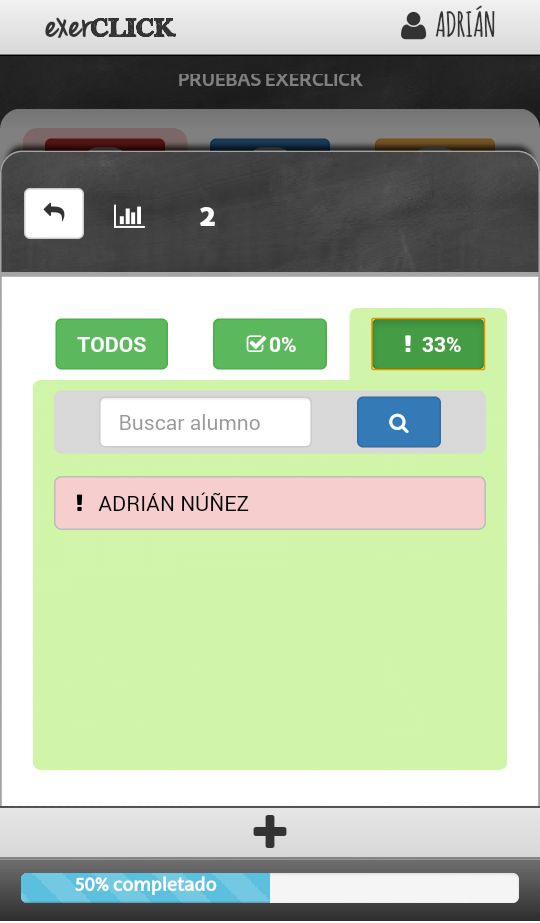
\includegraphics[height=7cm, frame]{P5D}
	\caption{P5D}
	\label{fig:fsm-autenticacion}
\end{subfigure}

\label{fig:autenticacion}
\end{figure}

\subsubsection{UO5-T: Ver la descripción completa de un ejercicio}
\label{diseno-e-implementacion:interfaces:profesor:uo5-t}

\begin{figure}[H]
	\centering
	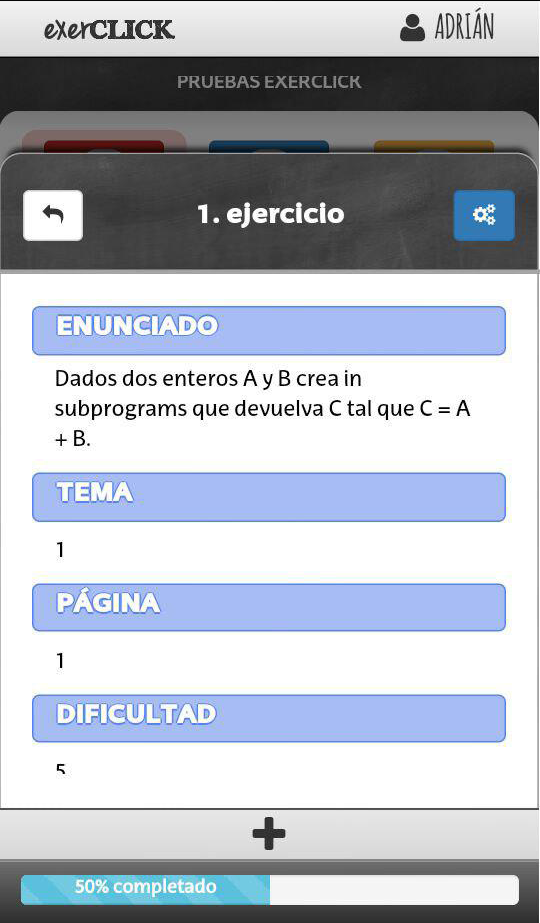
\includegraphics[height=7cm, frame]{P3}
	\caption{P3}
	\label{diseno-e-implementacion:interfaces:profesor:uo5-t:p3}
\end{figure}

\subsubsection{UO6-T: Editar un ejercicio}
\label{diseno-e-implementacion:interfaces:profesor:uo6-t}

\begin{figure}[H]
\begin{subfigure}[b]{0.3\textwidth}
	\centering
	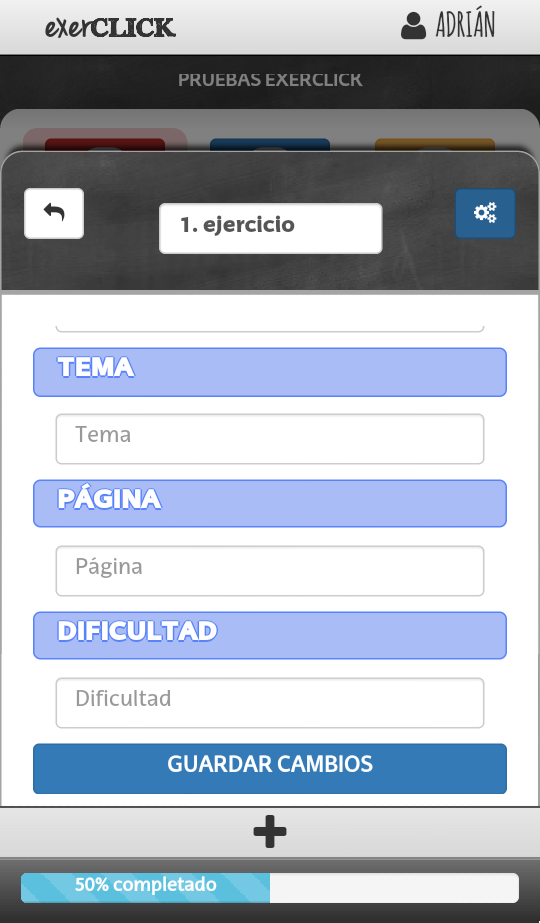
\includegraphics[height=7cm, frame]{P4}
	\caption{P5T}
	\label{fig:req-autenticacion:p0}
\end{subfigure}
%
\begin{subfigure}[b]{0.3\textwidth}
	\centering
	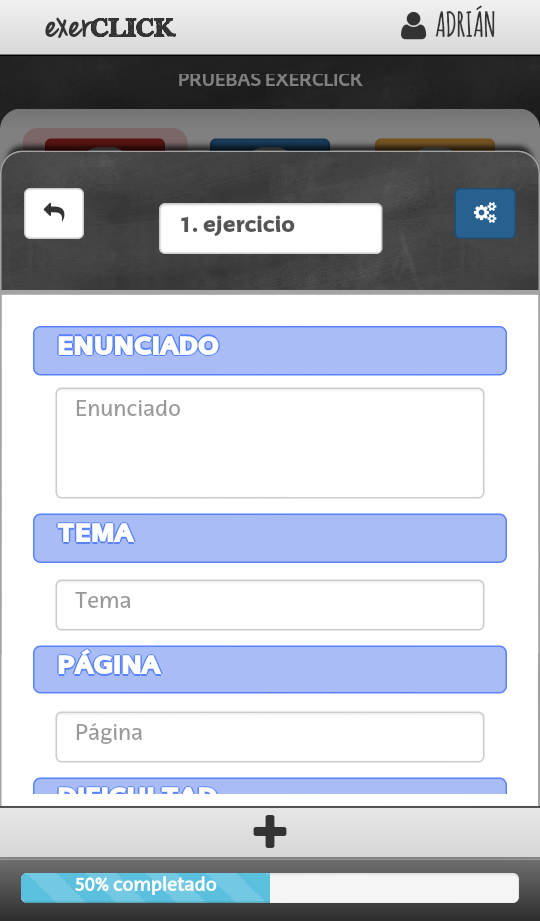
\includegraphics[height=7cm, frame]{P4-2}
	\caption{P5A}
	\label{fig:req-autenticacion:p0'}
\end{subfigure}
%
\begin{subfigure}[b]{0.3\textwidth}
	\centering
	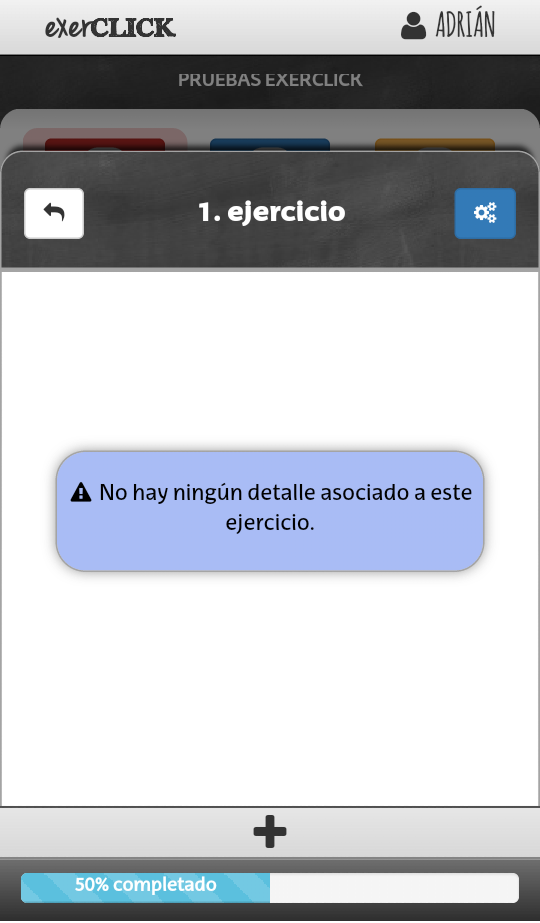
\includegraphics[height=7cm, frame]{P4'}
	\caption{P5D}
	\label{fig:fsm-autenticacion}
\end{subfigure}

\label{fig:autenticacion}
\end{figure}

\subsection{Interfaz del alumno}
\label{diseno-e-implementacion:interfaces:alumno}

AÑADIR IMAGEN DE LA VISTA ALUMNO.\\

La pantalla del alumno le muestra a este el estado actual de la clase: los ejercicios activos, su progreso en esta sesión y la media de progreso de la clase.

\subsubsection{UO1-S: Responder a un ejercicio}
\label{diseno-e-implementacion:interfaces:alumno:uo1-s}

AÑADIR IMAGEN UO1-S (dos, una con cada boton pulsado).

\subsubsection{UO2-S: Ver detalles de un ejercicio}
\label{diseno-e-implementacion:interfaces:alumno:uo2-s}

AÑADIR IMAGEN UO2-S.

\subsection{Uso de iconos mediante Font Awesome}
\label{diseno-e-implementacion:interfaces:font-awesome}

Font Awesome \hyperref[fontawesome]{\cite{fontawesome}} es un sitio web generado mediante un repositorio de Github. De este sitio se han obtenido todos los iconos de la aplicación: desde los iconos de los botones hasta el icono de usuario que aparece junto al nombre de usuario.\\

Su uso es sencillo, para añadir cualquier icono basta con añadir código como el de este ejemplo (para añadir el icono del avión de papel de los ejercicios activos):\\

\lstset{language=HTML}
\begin{lstlisting}[frame=single]
<i class="fa fa-paper-plane"></i>
\end{lstlisting}

Además podemos aumentar el tamaño del icono añadiendo clases del tipo fa-2x, fa-3x, etc. (aumentan por 2 y por 3 el tamaño del icono, respectivamente). También existe la opción de adaptarlo al texto que tiene cerca con fa-fw y otras tantas opciones que no se han llegado a utilizar en el proyecto (rotaciones, añadir un marco de prohibido encima, etc.). Se pueden encontrar ejemplos en la propia página.\\

\section{Lógica de negocio o lado del servidor}
\label{diseno-e-implementacion:logica-negocio}

Hablar sobre la parte de servidor y la base de datos.\\

\subsection{Base de datos}
\label{diseno-e-implementacion:logica-negocio:bd}

El diseño de la base de datos se ha realizado considerando desarrollos anteriores del grupo GaLan.
Por ello muchos de los elementos son comunes con una de sus herramientas genérica de creación
de sistemas docente, MAGADI, que ha sido proporcionada para este proyecto.\\

Se han incorporado unas tablas nuevas a la base de datos ya existente para la gestión de ejercicios tal y como se muestra en la figura ~\ref{fig:base-de-datos} del apéndice C.\\